\chapter{Discussion}\label{chap:discussion}

This chapter presents a reflection on both the development process and the final product. It examines how the project evolved in relation to the original goals, highlighting what worked well, what could have been improved, and the challenges encountered along the way. The chapter discusses the choice of technologies, project management practices, and team collaboration. It also evaluates the effectiveness and limitations of the final solution, comparing it with existing alternatives and identifying unexpected findings. Broader considerations, such as sustainability and the role of AI in the project, are explored. Finally, the chapter outlines potential directions for future work and improvements to both the product and the project approach.

\section{Process}\label{sec:discussion:process}

This section provides a reflection on the project's development process, covering both planning and execution. It examines how the initial project plan guided the work, the technologies that were selected, and the software development methodology that was followed. The section also evaluates the collaboration within the group, including how communication was handled and how responsibilities were distributed. In addition, it highlights areas where the process could have been improved, and describes how AI tools were used throughout the project to support development, planning, or writing tasks.

\subsection{Project Plan}\label{subsec:discussion:process:projectplan}

Looking back, we were able to mostly follow the project plan, but there were certain tasks that either were rescheduled or removed entirely for practical reasons. The most difficult part of planning was knowing how much time to allocate to each part of the project. There were multiple times where we had either worked faster than expected or had to postpone tasks due to unforeseen issues. Using tools like Planning Poker could have made this easier. The goal of the method is to make estimations individually without being influenced by the other group members \cite{planningpokerwiki}. Additionally, our time estimations were based on high-level task descriptions, which proved too abstract. Breaking tasks down into more granular, concrete sub-tasks could have led to more accurate and realistic estimates.

One of the biggest strengths of the project plan was the structure provided by Scrum and the use of sprints. The plan's division into eight sprints allowed us to stay focused and iterative, and it gave us frequent opportunities to re-evaluate priorities and progress. However, we found that the sprint content sometimes had to be adjusted mid-way through to accommodate emerging challenges, such as unexpected bugs, changes between data sources, or new feature requests from the Product Owner. Knowing this, the sprint length could potentially have been shorter, e.g., the first few sprints were 1-week then the later ones could have been 2-weeks. 

Our Gantt chart helped define clear milestones, like the MVP, and these helped us stay aligned with deliverables. Nevertheless, actual progress often did not align perfectly with the chart. For instance, early on we had a whole sprint for research, data collection and system design. In hindsight we only needed half a sprint for this and therefore we started designing the website which was planned for the next sprint. In later sprints we had planned user tests which kept getting pushed back, and in the end the formal user tests were replaced with feedback from the Product Owner and a presentation of the product for potential stakeholders.

The inclusion of the vacation in the plan was helpful, and having accountability measures, like compensating for delays by using it as a buffer, proved valuable in practice. The group contract and routine rules also helped maintain consistent effort and communication.

Another challenge we faced was scope control. As anticipated in the risk analysis (see \autoref{appendix:project_plan}), there was some pressure to expand the scope by including additional features or data sources. For example, the Product Owner emphasized that the product should at least function reliably in the local area (Gjøvik), but the final version ended up supporting the entire country. While this broader scope added value, it also introduced complexity and potential performance issues. Regular sprint meetings with our supervisor were essential in helping us manage these demands, keeping the project aligned with its core goals and preventing uncontrolled feature creep.

\subsection{Technologies}

This section contains a reflection of the different technologies and tools used throughout the project. We discuss both the client-side and server-side components, as well as supporting tools that contributed to collaboration, version control, and project management. The chosen technologies were selected based on factors such as ease of integration, documentation quality, performance, and our team's familiarity with them, or lack thereof.

\subsubsection{Website}

The chosen technologies for the website, TypeScript, React, and OpenLayers, proved to be well-suited for the project. Although we had little prior experience with these tools, their extensive documentation allowed us to quickly learn them throughout the development process.

While the overall scope of the application is moderate, using TypeScript instead of JavaScript improved type safety and reduced the likelihood of runtime errors. This added confidence during development and helped maintain code quality.

We had limited prior experience with web development, so we cannot directly compare React to building a website without a similar library. However, React's component-based structure made it easy to build and reuse interface elements, which likely made the development process more efficient and maintainable.

When selecting a map library, we evaluated several options, including more widely used ones like Leaflet and Mapbox. While these libraries are known for their ease of use and strong community support, we ultimately chose OpenLayers due to its built-in GIS functionality and flexibility. Unlike MapBox, OpenLayers is fully open-source and free to use, without licensing restrictions. In hindsight, while OpenLayers has a steeper learning curve, its comprehensive feature set allowed us to implement advanced functionality, such as WMS layers and raster overlays, without relying on third-party plugins, as would have been necessary with Leaflet.

\subsubsection{Server}

As described in \autoref{chap:implementation}, we made good use of the advantages of Go. Our prior experience with Go allowed us to implement advanced optimization techniques like multi threading and clustering. Consequently, the time spent developing the server was shorter compared to the website, as less time was used reading documentation and exploring unfamiliar frameworks.

Go's extensive package registry\footnote{\url{https://pkg.go.dev/}} of open-source libraries were vital for implementing certain functionality. Without the packages go-shapefile and go-geom, the superficial data could not have been stored locally and would have to have been sourced from an \acrshort{api}. This would lead to extensive processing times, as we query every \qty{10}{\meter} of road, and an external \acrshort{api} is considerably slower than in-memory data.

\subsubsection{Other Technologies}

\textcolor{orange}{traggo, docker, skyhigh etc.}

The use of GitHub for both version control and task management via the Kanban board\footnote{\url{https://github.com/orgs/skogkursbachelor/projects/1}} made it easy to track progress and adjust tasks as needed. This complemented the Scrum framework well and allowed us to keep the project transparent and adaptable. Storing everything in GitHub within its own repository proved to be very useful, as it allowed us to keep all project files in one centralized location. By backing up all documentation and diagrams, we ensured that nothing would be lost and provided easy access for all group members. Additionally, we decided to separate the frontend and backend into distinct repositories. This approach enhanced maintainability, since the frontend and backend are written in different programming languages and are deployed differently.

Using Traggo for time tracking made it straightforward to categorize work using tags. As a self-hosted and free solution, it did not require creating additional user accounts, which made access simple and efficient. It included all the core features we needed, though it lacked some useful extras, such as the ability to filter by multiple tags at once. For example, it was not possible to easily see how much time a specific user spent on a particular task.

\subsection{SDLC Model / SCRUM}

\textcolor{orange}{NOE TEKST}

\subsection{Communication}

The communication between the group members was consistently productive throughout the project. Knowing each other personally prior to the project allowed us to be blunt and precise during discussions, keeping the collaboration efficient, calm, and productive.

\gls{productowner} and our supervisor ...

\subsection{Work Allocation}

\textcolor{orange}{blabla}

\autoref{tab:timetrackedbymember} shows the total time of work for each month by the two members.

\begin{table}[h]
    \centering
    \begin{tabular}{c|c|c|c}
        \hline
        \textbf{Month} & \textbf{Bjørnsen} & \textbf{Houmb} & \textbf{Total} \\
        \hline
        January  & 61h 39m  & 62h 58m  & 124h 37m \\
        February & 80h 6m   & 79h 17m  & 159h 24m \\
        March    & 88h 4m   & 88h 20m  & 176h 24m \\
        April    & 99h 40m  & 102h 38m  & 202h 18m \\
        May      &        &        &        \\
        \hline
        Total & & & \\
        \hline
    \end{tabular}
    \caption{Tracked time by month and group member}
    \label{tab:timetrackedbymember}
\end{table}

% Skriv mer om time fordeling, f.eks. hvorfor mer timer i mars enn januar etc.

\autoref{fig:time_tracking_by_type} shows the total time of work for each month by the two members.

% KANSKJE IKKE TA SKJERMBILDE, LAG HELLER CHART MED LATEX f.eks. (pfg-pie).
% tar screen på mac for bra oppløsning
\begin{figure}[h]
    \centering
    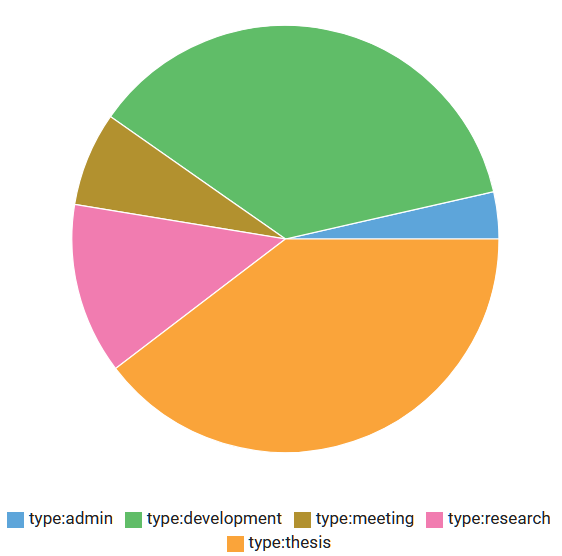
\includegraphics[width=0.5\linewidth]{figures/traggo_pie_chart_by_type.png}
    \caption{Pie chart of time spent in total per work type}
    \label{fig:time_tracking_by_type}
\end{figure}

\textcolor{orange}{OPPDATER PIECHART OG TABLL FØR LEVERING}

% SKRIV OM TIDSFORDELING FOR DE FORSKJELLIGE OPPGAVENE (THESIS, DEV, osv.)

\subsection{Improvements}

\textcolor{orange}{Hvordan forbedre tidsestimering? mangel på formell brukertesting? }

\subsection{Use of AI}

\textcolor{orange}{NOE TEKST}

\subsubsection{Learning}

\subsubsection{Inspiration}

\subsubsection{Spellcheck}



\section{Product}

\subsection{Goal Assessment}

\textcolor{orange}{blabla revisit the goals from \autoref{chap:requirements}}

\subsubsection{Product Goals}

The primary goal of the project was to develop and test a \textbf{prototype system for fully digital modeling of forestry road load-bearing capacity under varying conditions throughout the year.} 

\\ \textcolor{orange}{Siden det ikke var satte krav for produktet annet en det over, valgte vi å definere tasks selv som ville gi en pekepin på hva vi har oppnådd med sluttproduktet: marked in \textbf{bold}}


\textbf{Decide and gather relevant geological and meteorological data, which may include superficial deposits, soil moisture, ground water, and ground frost} 

The product integrates various geological and meteorological data sources, as described in \autoref{chap:mapdatasources}. Historical, real-time and forecast values for frost and soil moisture are available alongside superficial deposit data.

\textbf{Identify and implement suitable data sources and APIs for continuous updates.} 

As described in \autoref{chap:implementation}, data is sourced from various providers which required different approaches to incorporate in the application.

\textbf{Develop a rule-based model to classify road conditions based on environmental factors.}

\textbf{Extend the model to provide a forecast of road conditions at least a week in advance.}

\textbf{Design and develop an interactive map-based website for intuitive accessibility.}

\textbf{Implement a GIS-based visualization with real-time updates and historical road condition tracking.}

\textbf{Ensure that the system is optimized for transport managers, with a user-friendly interface that allows efficient decision-making.}

\textbf{Evaluate the accuracy and usability of the system by testing with real-world data.}

\textbf{Conduct user testing with transport managers or forestry stakeholders to assess the effectiveness of the interactive interface and forecasting capabilities.}

\textbf{Incorporate potential user feedback.}


According to the feedback we received from stakeholders, the product was intuitive and easy to use. The traffic-light system used to display road trafficability was especially well-received, as it provided a clear and familiar visual language. While the overall feedback was positive, some usability improvements were suggested. For example, although users could adjust the threshold values used in road classification, they wanted the ability to customize these values for specific roads or locations. Additionally, these thresholds should persist between sessions to avoid repetitive configuration.

\subsubsection{Impact Goals}

The project aimed to deliver real-world value by improving decision-making processes related to forestry road usage. The following impact goals outline the intended benefits for end-users and stakeholders:

\begin{itemize}
    \item Reduced uncertainty for transport managers when setting the routes using forest roads.
    \item To validate the prototype's feasibility and effectiveness by conducting tests with end-users, such as transport managers, to assess its performance and usability in real-world scenarios.
\end{itemize}

\subsubsection{Learning Goals}

In addition to delivering a functional prototype, the project served as a valuable learning experience. The goals below reflect the desired technical and professional growth for the project participants:

\begin{itemize}
    \item Gaining insight in implementing interactive maps and geospatial data on web pages.
    \item Leveraging RESTful APIs for efficient data integration.
    \item Acquiring hands-on experience collaborating with real-world companies and products.
    \item Gaining experience working in a team environment, improving collaboration and communication skills.
    \item Conducting user tests and implementing feedback. XXX
    \item Developing a deeper understanding of the software development life cycle while actively practicing agile methodologies, like Scrum and Kanban.
    \item Enhancing application performance by implementing concurrency and optimizing parallel processing.
    \item Expanding proficiency in containerization techniques, particularly through hands-on experience with Docker.
\end{itemize}

\subsection{Limitations}

% Feilkilder (kartdata) e.g. https://www.senorge.no/WaterMap
% Vanskelig å få tilgang til satellittdata fra SMAP & SENTINENTAL-1. For å få prognose må man ha en modell for å regne ut.

\textcolor{orange}{- Bad performance when a lot of vector features are rendered on the screen, this also differs from monitor resolution. - Not HTTPS: security issues, can't use geolocation, etc.}

\subsection{Comparison with Existing Products?}

\textcolor{orange}{NOE TEKST}

\subsection{Unexpected Findings} % Kanskje fjern?

\textcolor{orange}{NOE TEKST}

\subsection{Sustainability}\label{subsec:discussion:product:sustainability}

This section explores the sustainability implications of the developed product, with a focus on environmental, economic, and social dimensions. It begins by applying a simplified version of the \acrfull{susaf} to identify and analyze the product's potential impacts across different levels, from immediate operational effects to long-term structural changes. The section then relates these findings to relevant United Nations Sustainable Development Goals (SDGs). Finally, the discussion is divided into three subsections, economic, social, and environmental, each examining how the product aligns with specific \acrshort{sdg} targets and what implications this may have for sustainable forestry and responsible technological development.

\subsubsection{Sustainability Awareness Framework}\label{subsubsec:discussion:product:sustainability:susaf}

To assess the sustainability of the product, a simplified version of the \acrfull{susaf} was applied. This framework serves as a tool to identify potential sustainability impacts by guiding the analysis through a series of structured questions. These questions are typically grouped into five dimensions: social, individual, environmental, economic, and technical. However, in the simplified version used here, the social and individual dimensions are combined into a single category: human sustainability \cite{ntnususaf}. Each team member reviewed relevant aspects of the product and identified possible sustainability effects by answering the structured questions and selecting the most important effects by likelihood and impact. \textcolor{orange}{One such.... høres ut som man skal utdype noe om det spørsmålet, kanskje?}. One such question from the environmental dimension was: "How can the product or service create or destroy monetary value?" \cite{susosusaf}.

The next step is to construct chains of effects to understand how the product may influence sustainability over time. This involves determining the orders of effect, which categorize consequences into three levels: immediate, enabling, and structural. Immediate effects refer to direct consequences from the production, operation, use, or disposal of the system. Enabling effects are changes made possible by the system's operation or use. Structural effects represent deeper, systemic changes, such as shifts in norms, policies, or legal frameworks, driven by the system's ongoing presence and influence \cite{susosusaf}.

Once the effects are identified and categorized, they are linked to form chains of effects, as illustrated in the Sustainability Awareness Diagram (see \autoref{fig:susafdiagram}). This diagram visualizes how one effect can lead to another, helping to uncover both short- and long-term sustainability consequences \cite{susosusaf}.

\begin{figure}[h]
    \centering
    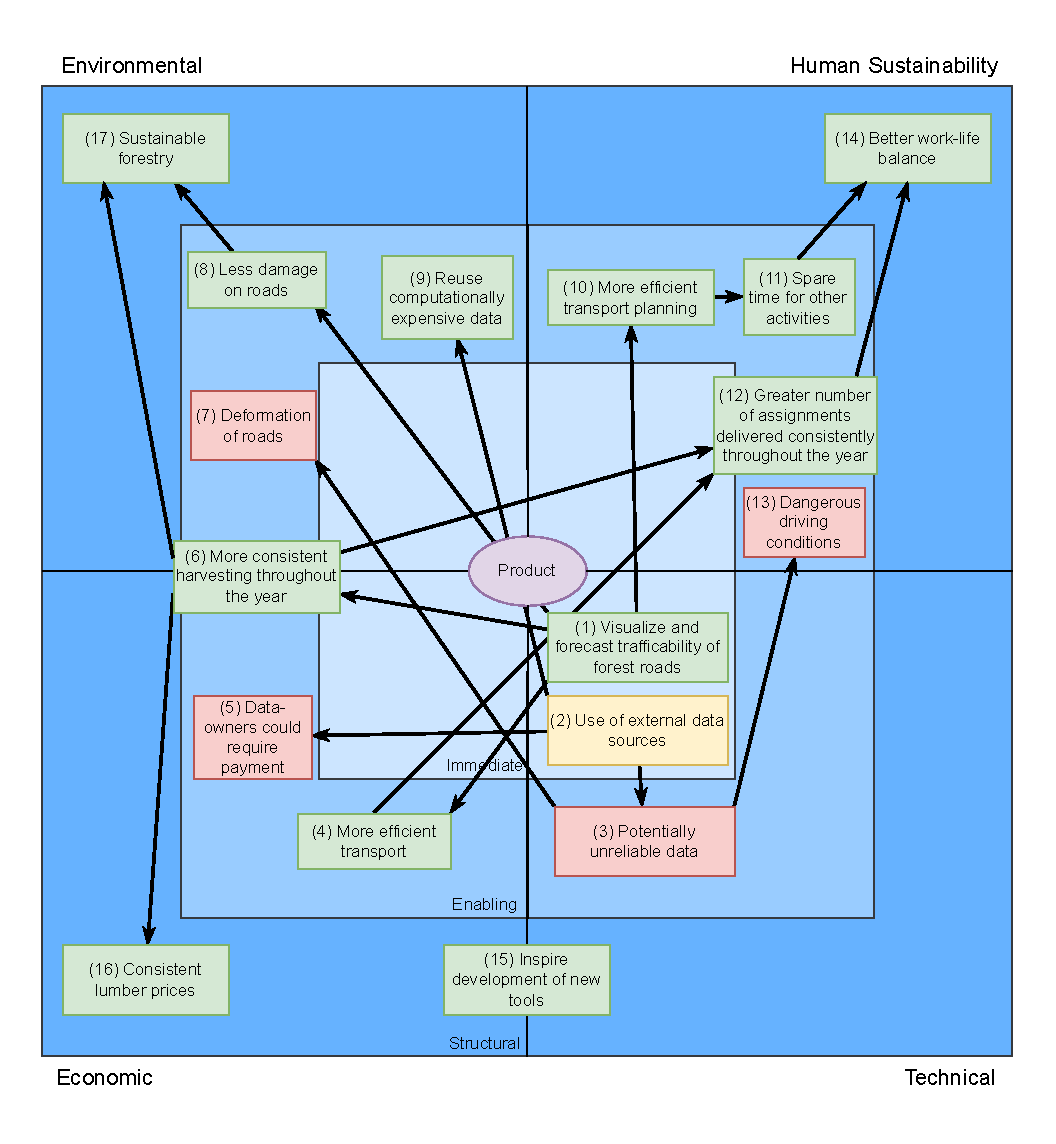
\includegraphics[width=0.8\linewidth]{figures/susaf.pdf}
    \caption{Sustainability Awareness Diagram}
    \label{fig:susafdiagram}
\end{figure}

From the analysis, two chains of effects leading to structural change were found. An immediate effect of the product is that it provides a way to visualize and forecast trafficability of forest roads. This enables more consistent harvesting throughout the year, which could lead to the structural change of more consistent lumber prices and sustainable forestry. The other chain also starts from the same immediate effect and leads to sustainable forestry, but by enabling less damage on roads.

Some potentially negative chains of effects were also identified. The reliance on external data sources introduces certain risks. For instance, data providers may begin charging for access, which could impact the product's long-term viability. Additionally, since the data is controlled by third parties, it may be incomplete, outdated, or otherwise unreliable. This could, in turn, lead to incorrect assessments of road conditions, potentially resulting in hazardous driving situations or damage to forestry roads. The different chains of effects are detailed in \autoref{tab:chain_of_effects}.

\begin{table}[h]
    \centering
    \renewcommand{\arraystretch}{1}
    \begin{tabularx}{\textwidth}{|l|X|l|l|l|}
        \hline
        \rowcolor{gray!20}
        \textbf{ID} & \textbf{Effect} & \textbf{Level} & \textbf{Affects} & \textbf{$+/-$} \\ 
        \hline
         1 & Visualize and forecast trafficability of forest roads & Immediate & 4, 6, 8, 10 & $+$ \\
         \hline
         2 & Use of external data sources & Immediate & 3, 5, 9 & $=$ \\
         \hline
         3 & Potentially unreliable data & Enabling & 7, 13 & $-$ \\
         \hline
         4 & More efficient transport & Enabling & 12 & $+$ \\
         \hline
         5 & Data owners could require payment & Enabling &  & $-$ \\
         \hline
         6 & More consistent harvesting throughout the year & Enabling & 12, 16, 17 & $+$ \\
         \hline
         7 & Deformation of roads & Enabling & & $-$ \\
         \hline
         8 & Less damage on roads & Enabling & 16 & $+$ \\
         \hline
         9 & Reuse of computationally expensive data & Enabling & & $+$ \\
         \hline
         10 & More efficient transport planning & Enabling & 11 & $+$ \\
         \hline
         11 & Spare time for other activities & Enabling & 14 & $+$ \\
         \hline
         12 & Greater number of assignments delivered consistently over the year & Enabling & 14 & $+$ \\
         \hline
         13 & Dangerous driving conditions & Enabling & & $-$ \\
         \hline
         14 & Better work-life balance & Structural & & $+$ \\
         \hline
         15 & Inspire development of new tools (Affected by all positive effects) & Structural & & $+$ \\
         \hline
         16 & Consistent lumber prices & Structural & & $+$ \\
         \hline
         17 & Sustainable forestry & Structural & & $+$ \\
         \hline
    \end{tabularx}
    \caption{Table showing chain of effects}
    \label{tab:chain_of_effects}
\end{table}

From this analysis, the product's effect on sustainability can also be related to the UN \acrshort{sdg}s. These goals are split into three dimensions, economic, social, and environmental. \textcolor{orange}{nevne at wedding cake er brukt?}

\begin{comment}
LENKE FRA PETER: https://www.ntnu.edu/web/excited/sustainability-in-computing-education
% Står litt om skogkurs og bærekraft: https://s46339.pcdn.co/wp-content/uploads/Sluttrapport.pdf
% OG HER: https://skogkurs.no/fagartikler/baerekraftige-metoder-og-kompetanse-i-skogsmaskinbransjen-kurs-kommer/ ->
- mer lukkede hogstformer og mindre bruk av flatehogst 
- **lavere drivstofforbruk og smartere kjøring med skogsmaskin** 
    - **lavere førerbelastning**
    - **mindre terrengslitasje**
    - **høyere produktivitet**
- produsere tømmer som er mest mulig tilpasset industriens behov 
- **videreutvikle teknologi for driftsoppfølging og førerstøtte for maskinførerne** 

###########################
FNs Bærekraftsmål som virker relevante (KANSKJE SAMMENLIGN MED HVA NORGE GJØR I DAG?):

- 9
- 12 (?) VIRKER SOM DEN FOKUSERER MEST PÅ UTVIKLINGSLAND?
- 15 (?)
\end{comment}

\subsubsection{Economic}\label{subsubsec:discussion:product:sustainability:economic}

% 9.5 Enhance scientific research, upgrade the technological capabilities of industrial sectors in all countries, ...
%\textcolor{orange}{SDG: 8 (8.2, 8.4), 9 (9.5)}
%\textcolor{orange}{Your product contributes directly to improved economic productivity by making forestry logistics more data-driven and efficient (effects 1, 4, 6, 11, 13). By enabling better forecasting of trafficability, it supports more consistent harvesting and delivery schedules, which benefits forestry operations financially and operationally. This aligns with Goal 8.2, as you're using digital innovation to enhance productivity in a traditional sector.\\ The reuse of data (effect 10) and reduction in road damage (effect 9) both support resource efficiency (Goal 8.4), helping reduce unnecessary fuel usage, road maintenance, and inefficient trips.\\The system as a whole enhances technological capability within the forestry sector, directly aligning with Goal 9.5.}

Visualizing the trafficability of forestry roads enhances the efficiency of lumber transport from logging sites by facilitating better planning and decision-making. It reduces uncertainty about the trafficability of specific roads, also helping to prevent damage and deformation caused by driving during unsuitable conditions. These improvements align closely with the United Nations' \acrshort{sdg}s, particularly Goal 8 (Decent Work and Economic Growth) and Goal 9 (Industry, Innovation, and Infrastructure). 

Target 8.2 is the following: "Achieve higher levels of economic productivity through diversification, technological upgrading and innovation, including through a focus on high-value added and labour-intensive sectors", with the indicator of annual growth rate of real GDP per employed person \cite{sdgsgoals}. Effect number 4, 6, and 12 (see \autoref{tab:chain_of_effects}) are relevant to this indicator by making parts of the forestry industry more efficient, by upgrading the technological tools used. Similarly, target 9.5 is: "Enhance scientific research, upgrade the technological capabilities of industrial sectors in all countries, ...", with the indicators of research and development expenditure and amount of researchers per million inhabitants \cite{sdgsgoals}. A possible side-effect of all positive effects is that they inspire industrial sectors to increase expenditure and focus on research and development of data-driven tools make specific tasks more effective, as described in effect 15.

\subsubsection{Social}

\textcolor{orange}{Kanskje si man mangler her, og nevn hvordan det kunne forbedres. SDG: 10 (10.2 [usability]), 3.6 [trafikkulykker], 8 [stable life-work balance?] skriv om første setning?}

By making the planning of transport routes more efficient the product may contribute to more predictable work schedules and a reduced need for overtime, leading to a better work-life balance, as described in effect number 14. These improvements relate to both \acrshort{sdg} 8 (Decent Work and Economic Growth) and \acrshort{sdg} 3 (Good Health and Well-Being). A better work-life balance supports healthier working conditions and can improve mental well-being. This is especially relevant in Norway, where recent editions of the World Happiness Report indicate a decline in overall happiness. Increased stress at work can negatively affect mental health and, by extension, impact national well-being scores \cite{sdg3no}.

\subsubsection{Environmental}

\textcolor{orange}{SDG: 15 (15.2, 15.b), 12 (12.2). Nevnt mulig "Rebound effect" fra at det blir lettere å frakte tømmer, kanskje?}

As Effect 6 from the \acrshort{susaf} says, the product contributes to more consistent harvesting and reforestation practices, supporting the development of sustainable forestry. This aligns with the United Nations' \acrshort{sdg} 15.2, which focuses on promoting sustainable management of all types of forests \cite{sdgsgoals}.

Furthermore, the product supports \acrshort{sdg} 12, particularly target 12.2, which emphasizes the sustainable management and efficient use of natural resources \cite{sdgsgoals}. By reducing road damage through better trafficability planning (effect 8), the product also helps prevent unnecessary wear on transport vehicles and minimizes environmental disturbance caused by repeated repairs or rerouting.

As stated in \autoref{subsubsec:discussion:product:sustainability:economic}, the product may inspire further innovation in the forestry sector. This applies to \acrshort{sdg} 15.b, which calls for mobilizing resources to finance sustainable forest management and promote the development of related technologies and initiatives \cite{sdgsgoals}.

% Jevons paradox https://en.wikipedia.org/wiki/Jevons_paradox
% Mer effektiv, mer etterspørsel -> Mer hogst -> if {ikke blir planta ny skog} = unsustaiable forestry

Not all aspects of the product necessarily contribute to greater sustainability. A relevant consideration is the Jevons paradox, which  occurs when technological advancements make a resource more efficient to use, however, as the cost of using the resource drops, if the price is highly elastic, this results in overall demand increasing, causing total resource consumption to rise \cite{jevonsparadoxwiki}. In this context, by making lumber harvesting more efficient, the product may contribute to lower prices and increased demand for lumber. If this demand is not met with a corresponding increase in reforestation efforts, it could result in unsustainable forestry practices.

\subsection{Future Work}

Throughout the project, the application has evolved with the most prioritized features being implemented. The group has considered various ideas for additional functionality, and we have also received valuable feedback from the Product Owner and other stakeholders. However, due to time constraints, several of these suggestions were not incorporated during the project period. Below is a list of some of these ideas:

\begin{itemize}
    \item \textbf{User Guide}: Include a user guide on the website on how to use it.
    \item \textbf{Mobile Application}: Implement for better use on mobile devices.
    \item \textbf{Offline Mode}: Download map data for a set time period and location. This requires that the application is deployed as a mobile or desktop application.
    \item \textbf{Export Data}: Let the user export data (e.g., CSV) for use in other applications.
    \item \textbf{Machine Learning}: Use machine learning to improve predictions about trafficability.
    \item \textbf{Notification System}: Send notifications or webhooks for changes in trafficability or weather.
    \item \textbf{Reporting System}: Generate reports that show the state of forestry roads in a period. Could include diagrams, statistics, etc.
    \item \textbf{Better Accessibility}: Better universal design. Color-blind modes and accessibility controls.
    \item \textbf{Hour Picker}: Updating the Data Picker component to also be able to select the hour of day could be useful if conditions vary a lot hourly, for example when the temperature oscillates around \qty{0}{\celsius} throughout the day. \textcolor{orange}{Noe mer om at veien blir bedre når den er kald, selvom frosten ikke er dyp.}
    \item \textbf{Performance}: Ways of improving performance. Using WebGL for rendering of vectors. This does require newer hardware/browsers) også backend opti). Performance testing flere brukere samtidig?
    \item \textbf{User Testing}: Conduct structured user testing.
    \item \textbf{Integrate with Existing Solutions}: Use with existing solutions like VSYS. 
    \item \textbf{Filtering}: Better ways of filtering by roads and locations.
\end{itemize}

\begin{comment}
    - User Guide
    - Offline Mode (download a map with data)
    - Mobile (har vi alt?)
    - Export Data
    - Machine Learning
    - Notification System
    - (Condition reporting system, si at en trucker kan si at denne veien var dårlig, typ det DF mente)
    - Better Accessibility (e.g. color-blind modes)
    - Hour picker (for mer detaljert data for spesifikke tidspunk, f.eks. om en sjåfør skal kjøre om natten)
    - More Optimization?
        - WebGL for rendering of vectors (downside?: does require newer hardware/browsers)
    - Code Quality, what to add to improve?
\end{comment}
